\documentclass[a4paper, 11pt]{article}
\usepackage{geometry}
\geometry{letterpaper, margin=1in}
\usepackage{amsmath}
\usepackage{amssymb}  
\usepackage{amsthm}
\usepackage{ulem} 
\usepackage{graphicx}
\graphicspath{ {images/} }
\usepackage{tikz} 
\usepackage{hyperref} 
\usepackage{movie15}

\begin{document}
%Header-Make sure you update this information!!!!
\noindent
\large\textbf{Complex Analysis - MTH 483} \hfill \textbf{John Waczak} \\
\normalsize Day 11 \hfill  Date: \today \\

\subsection*{Moving towards Cauhcy's Theorem... Primitives}
	\textit{Definition} let $f:\Omega\rightarrow\mathbb{C}$ be holomorphic. A \textit{primitive} a.k.a. anti-derivative for $f$ is a holomorphic function say $F:\Omega \rightarrow\mathbb{C}$ s.t. $F'(z) = f(z)$. \\
	
	\noindent\textit{Example} $f(z)=2z$ is holomorphic on $\mathbb{C}$ and $F=z^2$ is a primitive. \\ 
	
	\noindent\textit{Exmaple} let $\Omega = \mathbb{C}\setminus\{0\}$ and let $f(z)=\frac{1}{z^n}$ for $n\geq1$. 
		\begin{itemize}
			\item Case 1: $n\geq 2$ in this case $F(z)$ is $\frac{1}{-n+1}z^{-n+1} = \frac{1}{(1-n)z^{n-1}}$ is a primitive. 
			
			\item Case 2: if $n=1$ i.e. $f(z)=\frac{1}{z}$ does \textit{not} have a primitive on $\Omega = \mathbb{C}\setminus\{0\}$. However if we consider $\Omega=\mathbb{C}\setminus(-\infty, 0]$. On this region, $f(z)$ has $F(z)=Log(z)$. 
		\end{itemize}



\subsection*{Evaluating integrals with primitives}
	\textbf{Theorem} Let $f:\Omega \rightarrow\mathbb{C}$ be holomorphic with primitive $F$. Suppose we have a path $\gamma$ in $\Omega$. Then 
		\begin{equation*}
			\int_{\gamma} f(z)dz = F(\gamma(b))-F(\gamma(a))
		\end{equation*}
	\noindent \textit{pf}. $F'(z)=f(z)$. Use the F.T.C. with inverse chain rule in integrand. \\ 
	
	\noindent \textbf{Theorem} let $f:\Omega \rightarrow \mathbb{C}$ be holomorphic with primitive $F:\Omega\rightarrow\mathbb{C}$ and let $\gamma$ be closed curve in $\Omega$. Then $\int_\gamma f(z)dz = 0 $. pf use previous theorem. \\ 
	
	\noindent Now we see why $f(z)=1/z$ does not have a primitive on $\mathbb{C}\setminus\{0\}$. If it did, then we would have $\int_{|z|=1}\frac{1}{z}dz = 0$. This is wrong. In fact, let $\gamma(t) = e^{it}$ then $\int_0^{2\pi} = \frac{1}{e^{it}}ie^{it}dt=2\pi i \neq 0$. 


\subsection*{Homotopy - continuously deforming one curve into another}
	\textbf{Definition} let $\Omega$ be a region in $\mathbb{C}$ and let $\gamma_0, \gamma_1:[0,1]\rightarrow\mathbb{C}$ be two closed curves in $\Omega$. We say that $\gamma_0$ is $\Omega$-homotopic to $\gamma_1$ if $\exists$ continuous function $h:[0,1]\times[0,1]\rightarrow\Omega$ such that $h(t,0)=\gamma_0(t)$ and $h(t,1)=\gamma_1(t)$. Finally, we want $h(0,s)=h(1,s)$ for closure. \\
	
	\noindent Notaiton: $\gamma_0 \sim_\Omega \gamma_1$ signifies homotopy. 
	\begin{figure}[!hbt]
		\centering
		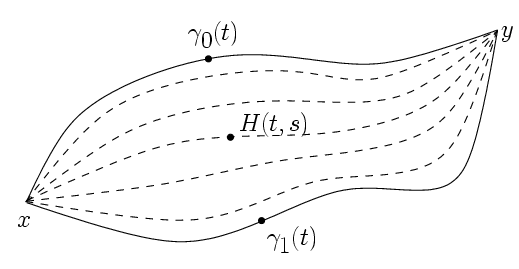
\includegraphics[width=0.35\columnwidth]{homotopy}
	\end{figure}
	
	\noindent\textbf{Theorem} Let $\Omega\subseteq\mathbb{C}$ be a region and let $f:\Omega\rightarrow\mathbb{C}$ be holomorphic. Let $\gamma_0 \sim_\Omega \gamma_1$ be curves in $\Omega$. Then 
		\begin{align*}
			\int_{\gamma_0} f(z)dz = \int_{\gamma_1} f(z)dz. 
		\end{align*}
 
 
 
 
 

	
\end{document}




































